\section{Үр дүн}

\begin{figure}
	\centering
	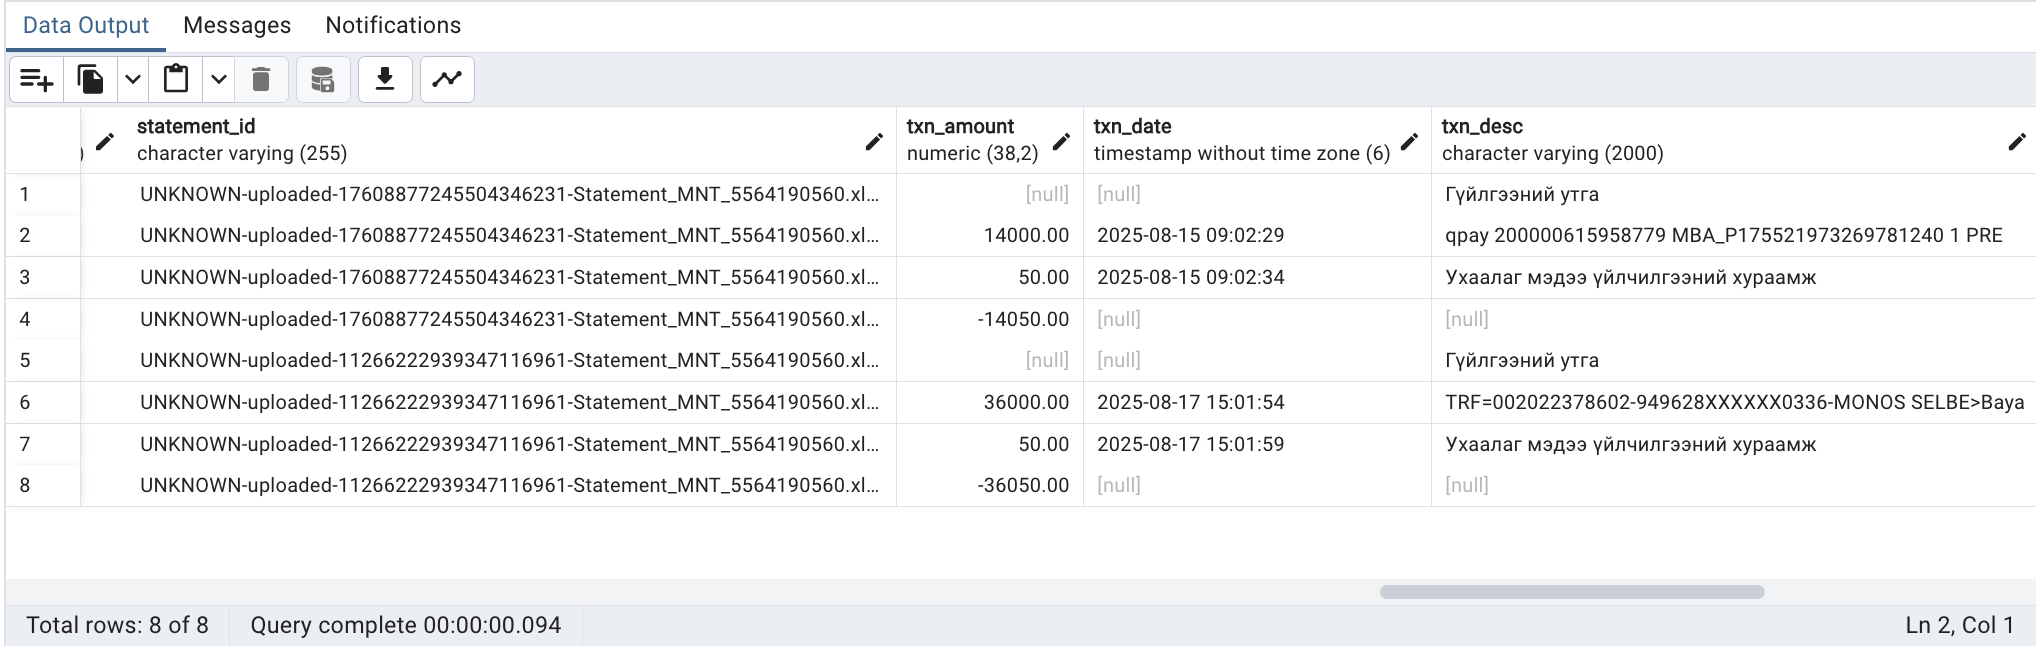
\includegraphics[width=15cm]{images/result.png}
	\caption{Гүйлгээний мэдээллүүдийг өгөгдлийн санд амжилттай оруулсан байдал}
	\label{fig:result}
\end{figure}
\pagebreak

\pagebreak
\section{Үр дүнгийн тайлан}
Монгол Ай Ди компанид 21 хоногийн хугацаанд үйлдвэрлэлийн дадлагыг хийснээр би онолын мэдлэгээ практиктай холбон, программ хангамжийн хөгжүүлэлтийн бодит орчинд туршлага хуримтлуулав. Энэ хугацаанд би байгууллагын технологийн багтай хамтран ажиллаж, баг хоорондын зохион байгуулалт, Agile зэрэг хөгжүүлэлтийн орчин үеийн арга зүйтэй танилцсан.
Дадлагын удирдагч, Технологи хариуцсан захирал Х. Ганзориг надад Java технологид суурилсан нэг модулийг сайжруулах ажлыг даалгасан. Би байгууллагын техникийн баримт бичгүүдийг судалж, өөрийн санааг нэмэн тухайн модулийг амжилттай сайжруулж, ашиглалтад өгөв. Энэ төсөл нь миний шийдвэр гаргах, асуудал шийдвэрлэх чадварыг дээшлүүлсэн юм.
Дадлагын эхэнд тавьсан программ хангамжийн загварууд болон хөгжүүлэлтийн арга барилуудыг судлах зорилгодоо хүрснээс гадна, өөрийн мэргэжлийн ирээдүйн чиг хандлагыг тодорхойлж, үүнд хүрэхэд шаардлагатай хувийн хөгжлийн төлөвлөгөөг гаргах боломжтой болсон. Энэхүү дадлага нь миний хувьд мэдлэг, ур чадвараа нэгтгэн, ирээдүйн карьертаа бэлтгэх чухал алхам боллоо.